\chapter{Metriken und Diagramme}
\label{cha:Metriken_Diagramme}

% Idee: Hervorheben wofür die Diagramm genutzt werden? Feature-Importance, ...

Dieses Kapitel beschäftigt sich mit der Analyse der einzelnen Diagrammtypen und\linebreak ihrer Implementierung in HeuristicLab \parencite{HeuristicLab}.
Hierbei wird zuerst untersucht welche Informationen in den Diagrammen visualisiert werden. Danach\linebreak erfolgt eine genaue Analyse jedes Diagrammtyps.
Das Ziel ist es herauszufinden, welche Informationen durch die Visualisierung gewonnen werden. Außerdem werden die Funktionalitäten der einzelnen Diagramme definiert. 
Diese dienen als Anforderungen an die Implementierung in Scikit-charts. Im weiteren Schritt werden diese Informationen\linebreak verwendet, um bestehende Bibliotheken mit HeuristicLab zu vergleichen.

\section{Metriken}
\label{cha:Metriken}

Die Metriken in HeuristicLab werden aus den Einträgen des Datensatzes und den\linebreak Vorhersagen gesammelt. Folgende Metriken können aus den einzelnen Diagrammen\linebreak erkannt werden:

\begin{description}
\item[Index] \hfill\newline
Die Position des Eintrages im Datensatz.
\item[Zielwert] \hfill\newline
Der beobachtete Wert der Zielvariable im Datensatz.
\item[Vorhersage] \hfill\newline
Der berechnete Wert des Regressionsmodells für die gegebenen Einflussvariablen.
\item[Residuum] \hfill\newline
Der Unterschied von Zielwert und Vorhersage (\cite{RegressionGrundlagen}).
\item[Relativer Fehler]  \hfill\newline
Das Residuum relativ zum Zielwert.
\item[Einflussvariablen] \hfill\newline %Features
Die Werte der Variablen im Datensatz, aus welchen das Regressionsmodell die Vorhersage berechnet. Im Englischen auch \textit{Feature} genannt.
\end{description}

\vspace{\baselineskip}

\noindent Residuum und Fehler haben außerdem einen zusätzlichen zweiten Eintrag, mit absoluten Zahlenwerten.

\section{Allgemeine Funktionen der Diagramme}
\label{sec:allgemeine_funktionen_diagramme}

Alle Diagramme, außer dem Schnittdiagramm, unterstützen ein Zoomen mithilfe der Maus. Dabei kann ein Bereich des Diagramms ausgewählt werden, um ihn über die gesamte Größe anzuzeigen. Durch einen Doppelklick mit der linken Maustaste wird der Bereich wieder zurückgesetzt.

%ToDo: Beschreibung der Informationen welche daraus gewonnen werden!

\section{Liniendiagramm (line chart)}
\label{sec:line-chart}

Das Liniendiagramm vereinfacht das Erkennen von Mustern im Verlauf der Daten. Durch den Vergleich von Zielwerten und Vorhersagen kann außerdem geprüft werden, ob sich dieser Verlauf im Modell widerspiegelt. Dadurch bietet sich das Diagramm für Datensätze mit gereihten Daten an.

\begin{figure}[H]
    \centering
    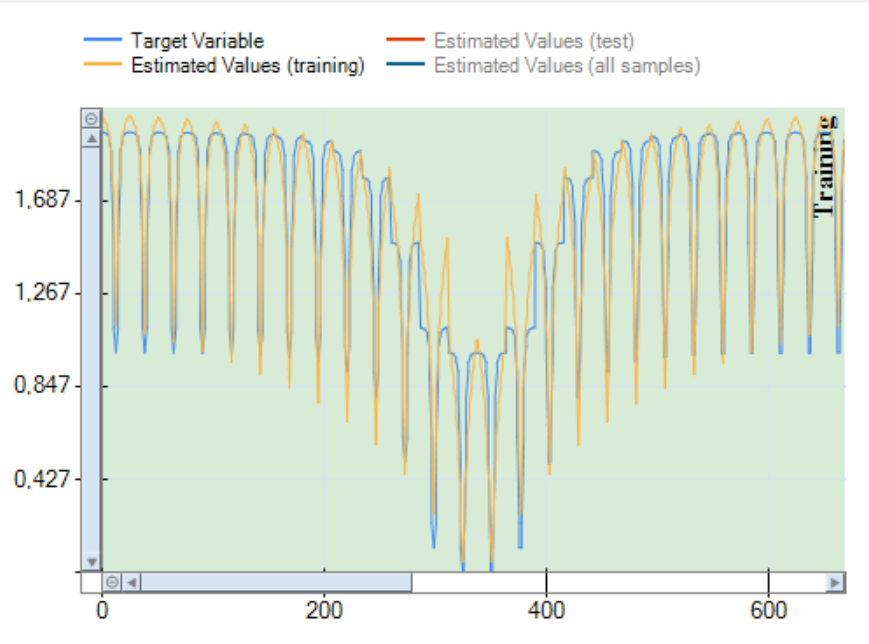
\includegraphics[height=.6\textwidth]{images/line-chart_small.png}
    \caption{Liniendiagramm in HeuristicLab}
    \label{fig:example_line_chart}
\end{figure}

\noindent Die Y-Achse gibt den Wertebereich der Zielvariable und der Prognosen an. Auf der\linebreak X-Achse ist der aufsteigende Index der Einträge angegeben.
Danach werden die Zielwerte und Vorhersagen als Punkte eingetragen und verbunden. Durch den Klick auf dem jeweiligen Namen kann die Anzeige der Werte aktiviert und deaktiviert werden.

\pagebreak

\section{Streudiagramm (scatter plot)}
\label{sec:scatter-plot}

Wie das Liniendiagramm dient auch das Streudiagramm zum Vergleich von Zielwerten und Vorhersagen. Die Reihenfolge der Beobachtungen im Datensatz, werden jedoch in diesem Diagramm ignoriert. Das Streudiagramm wird genutzt um zu prüfen,
ob es systematische Fehler in der Vorhersage der Werte gibt. Ist das nicht der Fall, sollten sich die Punkte der Geraden im Diagramm annähern.

\begin{figure}[H]
    \centering
    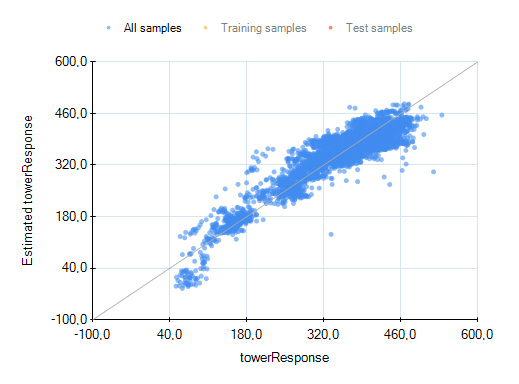
\includegraphics[height=.6\textwidth]{images/scatter-plot.png}
    \caption{Streudiagramm in HeuristicLab}
    \label{fig:example_scatter_plot}
\end{figure}

\noindent Die Y-Achse gibt den Bereich der Vorhersagen an. Auf der X-Achse sind die Zielwerte angegeben. Jeder eingetragene Punkt im Diagramm beschreibt die Überschneidung\linebreak dieser Werte. Die durchgehende Linie zeigt den Bereich an, auf welchem beide Achsenwerte ident sind.

\pagebreak

\section{Blasendiagramm (bubble chart)}
\label{sec:bubble-chart}

Das Blasendiagramm dient zur interaktiven Analyse der Zusammenhänge aller Variablen.
Er bietet sich also ebenfalls sehr gut an, um Fehler im Modell zu prüfen. Die dynamischen Interaktionen vereinfachen dabei die Analyse.

\begin{figure}[H]
    \centering
    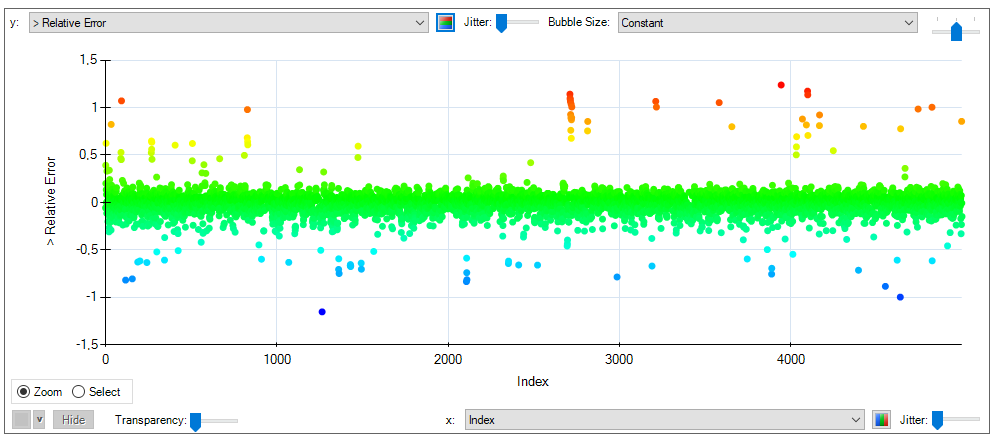
\includegraphics[height=.5\textwidth]{images/bubble-chart.png}
    \caption{Blasendiagramm in HeuristicLab}
    \label{fig:example_bubble_chart}
\end{figure}

\noindent Jede der aufgezeichneten Blasen zeigt einen einzelnen Eintrag im Datensatz. Die Variablen auf beiden Achsen können frei gewählt werden. 
Es ist ebenfalls möglich, einzelne Einflussvariablen auszuwählen.\newline\newline
Die Farben der Blasen können dynamisch gesetzt werden. Der Knopf neben der Metrik-auswahl setzt die Farben automatisch nach dem
Verlauf der Achse. In der Abbildung \ref{fig:example_bubble_chart} ist diese Färbung für die Y-Achse zu sehen. Außerdem ist es möglich, einen\linebreak Bereich von Blasen auszuwählen. Dieser kann danach explizit zu gefärbt oder ausgeblendet werden. Die Blasen behalten ihre Farbeinstellungen beim Wechseln der Metriken.\newline\newline
Die Jitter-Option neben der Metrikauswahl ermöglicht es, einen Versatz der gezeichneten Blasen einzustellen. Diese Option ist in beide Achsenrichtungen möglich.
Die Größe der einzelnen Blasen kann ebenfalls verändert werden. Die Option dafür ist in der rechten oberen Ecke zu finden. Der Wert der Größe kann konstant oder relativ zu einzelnen Metriken gesetzt werden. Zuletzt besteht ebenfalls die Option, die Transparenz der Blasen zu verändern.

\pagebreak

\section{Schnittdiagramm (partial dependency plot)}
\label{sec:partial-dependency-plot}

Das Schnittdiagramm dient zur Analyse der Zusammenhänge zwischen den Einflussvariablen und den Vorhersagen, die im Modell erfasst sind. Dadurch kann die Art der Abhängigkeit von Variablen als Funktion dargestellt werden. Diese Informationen\linebreak können für die Validierung und Plausibilisierung von Modellen helfen.

\begin{figure}[H]
    \centering
    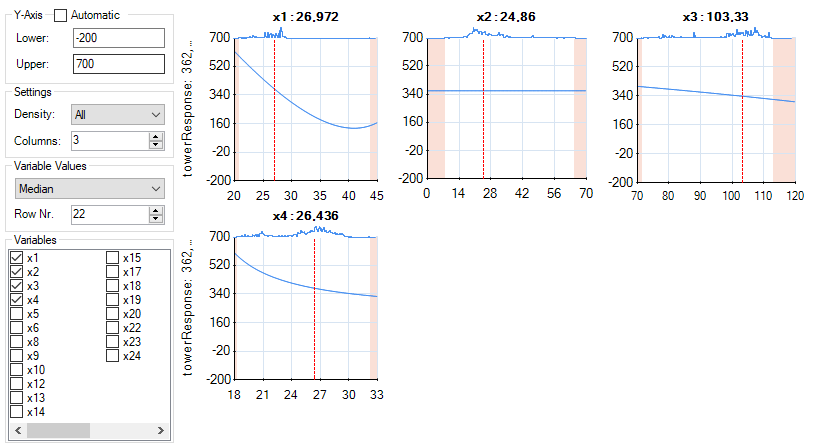
\includegraphics[height=.5\textwidth]{images/intersection-plot.png}
    \caption{Schnittdiagramm in HeuristicLab}
    \label{fig:example_partial_dependency_plot}
\end{figure}

\noindent Im rechten Bereich werden die Teildiagramme für die einzelnen Einflussvariablen abgebildet. Auf der Y-Achse werden die Vorhersagen dargestellt.
Die X-Achse repräsentiert die möglichen Werte der einzelnen Variablen. Die rot hinterlegten Bereiche befinden sich nicht im Datensatz,
sondern normalisieren den Wertebereich der Achse.
Die blaue Linie ist der Verlauf des Zusammenhangs zwischen Vorhersage und Variablenwert.\newline\newline
Der Text zu Beginn der Zeilen gibt den Wert der aktuellen Vorhersage an.
Im Titel steht der Name der Variable sowie ihr aktueller Wert. Dieser ist ebenfalls im Diagramm durch die rote Linie markiert. 
Diese Linie kann mit dem Mauszeiger verschoben werden. Dadurch werden sowohl Variablenwert, als auch die Vorhersage aktualisiert.
Die blaue Linie, oben an den Diagrammen, beschreibt die Dichte des Datensatzes über die X-Achse.\newline\newline
Im linke Bereich befinden sich Optionen um die Darstellung der Teildiagramme zu verändern. Dabei handelt es sich um den Wertebereich der Y-Achse und die Anzahl der Spalten im rechten Bereich. Außerdem kann der initiale Wert der Variablen in den Teildiagrammen gesetzt werden. Mögliche Werte sind der Median, der Durchschnittswert sowie bestimmte Zeilen im Datensatz. Die Diagramme können für einzelne Variablen aktiviert und deaktiviert werden.